\chapter{Training and First Results}
\label{ch:training}

% ---------------------------------------------------------------------------
% Part I record. Every number in this chapter is measured on data/v2 (legacy
% simulator, five corridors) with the first-generation surrogate, GNS-1.
% FROZEN: do not update after the v3 rebuild; Ch. 15 repeats this protocol.
% Sources: SURROGATE_FORMULATION_NOTE.md (development sweeps and the shape
% diagnosis, single seed, 2026-09-17) and the three-seed re-run of 2026-10-10:
%   python scripts/train_surrogate.py data/v2 --steps 6000 --budget-gib 5 \
%       --ood --seed {0,1,2} --save checkpoints/gns1_seed{s}.pt
%   python scripts/eval_gns1.py data/v2 checkpoints/gns1_seed*.pt \
%       --out results/gns1_ch9/eval.json
%   python scripts/time_gns1.py data/v2 checkpoints/gns1_seed0.pt
% ---------------------------------------------------------------------------

\Cref{ch:architecture} built a network that advances a consist by one fixed step of 0.25\,s. This chapter trains it and asks three questions of the result. Does it learn the step, so that one prediction from a true state is accurate? Does it stay accurate when it runs on its own predictions for hundreds of steps, which is how a controller will use it? And does it extrapolate, to consists longer than any it was trained on and to corridors it has not seen? The third question is the one the graph formulation was chosen to answer (\cref{sec:tensor_state_rep}).

Everything here is measured on \texttt{data/v2}, the corpus of \cref{ch:gpu_dataset}, generated by the simulator of \cref{ch:refsim} on the five corridors of \cref{ch:routes}. The model is the network of \cref{ch:architecture} and is called GNS-1 where it must be told apart from the revised model of Part~III. The chapter closes with a list of what these results claim. Part~II then examines what those claims rest on.

\section{Experimental setup}
\label{sec:train_setup}

\subsection{Data}

\Cref{tab:train_splits} lists the splits of \texttt{data/v2} that this chapter uses. Training and the three in-distribution splits share three corridors and consists of 10 to 80 vehicles. The three held-out splits each change one thing. \texttt{ood\_size} keeps the training corridors but uses only consists of 120 to 150 vehicles, so there is no overlap in length with training. \texttt{ood\_corridor} and \texttt{ood\_grade} are whole corridors never seen in training, but they hold every consist size from 10 to 150. A score on either therefore mixes a change of corridor with a change of length. To keep the two apart, both are also scored restricted to consists of at most 80 vehicles, the trained range.

\begin{table}[htbp]
    \centering
    \begin{tabular}{lrcl}
        \toprule
        Split & Scenarios & Consist size & Corridors \\
        \midrule
        \texttt{train}        & 4,043 & 10--80  & \texttt{route\_line0}, \texttt{route\_line3}, \texttt{route\_line4} \\
        \texttt{val}          & 517   & 10--80  & same three \\
        \texttt{test\_id}     & 496   & 10--80  & same three \\
        \texttt{ood\_size}    & 955   & 120--150 & same three \\
        \texttt{ood\_corridor} & 1,990 & 10--150 & \texttt{route\_line5} \\
        \texttt{ood\_grade}   & 1,999 & 10--150 & \texttt{route\_line2} \\
        \bottomrule
    \end{tabular}
    \caption{Splits of \texttt{data/v2} used in this chapter (\cref{tab:dataset_splits}). No consist in the library has between 81 and 119 vehicles.}
    \label{tab:train_splits}
\end{table}

The training split is larger than fits in GPU memory alongside the model, so each run loads a random subset that fills a 5\,GiB budget: about 1,950 of the 4,043 scenarios, or 2.5 million transitions. The subset is drawn independently for each random seed. Evaluation sets are subsampled the same way within a 3\,GiB budget.

\subsection{Batches of one consist size}

Consist size varies from 10 to 150, and padding every batch to the longest consist would spend most of each batch on empty positions, since short consists dominate the corpus. Instead, scenarios are grouped by consist size, 70 groups in the training split, and each batch is drawn from a single group, chosen with probability proportional to its number of transitions. Every batch is then a rectangular array with no padding and no mask, and the network, whose weights do not depend on consist size (\cref{sec:arch_network}), never sees the difference.

Training across all sizes at once also proved better than training on one. A development run on 42-vehicle consists alone reached 3.4 times the zero-output baseline on velocity; training on every size from 10 to 80 with the same architecture, and a third more updates, reached 7.8 times on a validation set spanning that range. The second run saw more data, 2.5 million transitions against 155,000, and more varied data, and it is the configuration used throughout.

\subsection{Optimization}

The loss is \cref{eq:arch_loss}. Each run takes 6,000 updates with the Adam optimizer, batches of 256 transitions, a learning rate decaying from $10^{-3}$ along a cosine schedule, and gradients clipped to a norm of 1. A run takes about three minutes on one RTX~4090, plus about 40\,s to load the data. Every result in \cref{sec:train_results} is reported over three runs with different random seeds, each with its own training subset, as a mean with the spread between seeds where it matters.

\subsection{Metrics}

Two kinds of error are reported.

\textbf{One-step error} is measured from a true state: the model makes one prediction, and it is compared with the stored next state. For velocity the quantity is the root-mean-square error of the predicted mean acceleration $\bar a_i$, in m/s$^2$, over every vehicle and transition. For shape it is the root-mean-square error of the stretch correction $c_j$, in millimetres, over every coupler and transition.

\textbf{Rollout error} is measured after the model has run on its own output for $k$ steps from one true state. At each horizon the error is the largest over the consist, of $|v_i - v_i^{\text{true}}|$ for velocity and of $|\delta_j - \delta_j^{\text{true}}|$ for stretch, and the reported figure is the median of that maximum over many starting points. The maximum over the consist is used because the quantities a controller acts on, the worst coupler force and the fastest vehicle, are maxima. The median over starts keeps a handful of extreme scenarios from setting the headline.

The shape correction needs one further remark. It is sparse: on 64\% of transitions every coupler's correction is below 50\,$\mu$m, and almost all of the signal lies in slack run-in and run-out events, with the largest per-transition correction reaching 4.2\,mm at the 90th percentile and 23.5\,mm at the 99th. A median statistic would measure only the quiet majority, where predicting exactly zero is unbeatable. An early version of the metric did exactly that and reported the model as nine times worse than zero while its root-mean-square error was 4.6 times better. Shape is therefore reported by root-mean-square error and tail percentiles, never by a median of the one-step correction.

\subsection{Baselines}

Three baselines need no training, and every model result is reported beside them.

\begin{itemize}
    \item \textbf{Zero output} predicts no change over the step: mean acceleration zero and no stretch correction. Over 0.25\,s a freight consist barely changes state, so this is a strong bar; its one-step error is the size of the learning target itself.
    \item \textbf{Hold} freezes the starting state for the whole of a rollout. It is the rollout counterpart of zero output.
    \item \textbf{Constant acceleration} repeats the previous step's true mean acceleration and stretch correction, one step or many. It uses one stored state more than the model is given, the state a step before the start, so it is slightly favoured.
\end{itemize}

One baseline is missing on purpose. A single step of the physics itself, fourth-order Runge--Kutta at 0.25\,s, diverges (\cref{tab:arch_anchor_velocity}), so there is no physics-only model to compare with at this step size. The residual MLP and the transformer ablation named in \cref{ch:intro} were not run in Part~I and are reported in \cref{ch:results2}.

\section{Keeping a rollout stable}
\label{sec:train_stability}

A model trained only to predict one step from true states sees, during training, only states the simulator produced. In a rollout it is fed its own output, and its small errors move it into states it has never seen, where it predicts worse and moves further off. This is the standard failure of learned step models (\cref{sec:graph_rollout_stability}), and the first model trained here showed it plainly (\cref{tab:train_noise_effect}). Within 20 steps, five seconds of simulated time, its velocity error exceeded that of simply freezing the state, and by 50 steps it had converged to that baseline. Its stretch error at 20 steps, 40.4\,mm, was more than five times that of holding the state.

\begin{table}[htbp]
    \centering
    \begin{tabular}{rrccc}
        \toprule
        Steps & Time & No noise & With noise & Hold \\
        \midrule
        1  & 0.25\,s  & 0.0052 & 0.0044 & 0.0155 \\
        5  & 1.25\,s  & 0.0517 & 0.0131 & 0.0669 \\
        20 & 5.00\,s  & \textbf{0.2272} & 0.0317 & 0.2002 \\
        50 & 12.50\,s & 0.4447 & 0.0622 & 0.4523 \\
        \bottomrule
    \end{tabular}
    \caption{Rollout velocity error, the largest over the consist in m/s (median over starts), with and without noise injection during training. Development runs of 3,000 updates, one seed, validation split. Without noise the model is worse than holding the state after about 20 steps.}
    \label{tab:train_noise_effect}
\end{table}

\subsection{Noise injection}

The remedy introduced with graph network simulators \cite{sanchez2020gns} is to corrupt the inputs during training. Each training state has Gaussian noise added to every vehicle's velocity and every coupler's stretch, and the target is then recomputed from the \emph{perturbed} state to the \emph{true} next state. The label is therefore the correction that carries a drifted state back onto the trajectory, not the step the model would have taken from a clean one, and training spends its effort learning to correct drift. Positions are not perturbed, since absolute position enters the model only through route lookup on a 10\,m grid, and the actuator states are exact and never drift. A unit test checks that a perturbed state advanced by its recomputed targets lands exactly on the true next state.

\Cref{tab:train_noise_sweep} sweeps the size of the velocity noise. The best value, 0.005\,m/s, is close to the model's own one-step velocity error, which is the prescription of \cite{sanchez2020gns}: perturb by about as much as the model will drift. Stretch noise is set the same way, at 1\,mm. With noise, velocity error at 20 and 50 steps falls about sevenfold, and the model beats holding the state at every horizon in both channels.

\begin{table}[htbp]
    \centering
    \begin{tabular}{lccccc}
        \toprule
        Velocity noise (m/s) & 1 step & 5 & 20 & 50 & One-step RMSE (m/s$^2$) \\
        \midrule
        0     & 0.0052 & 0.0517 & 0.2272 & 0.4447 & 0.0207 \\
        0.005 & \textbf{0.0044} & \textbf{0.0131} & \textbf{0.0317} & \textbf{0.0622} & 0.0216 \\
        0.01  & 0.0053 & 0.0147 & 0.0372 & 0.0709 & 0.0222 \\
        0.02  & 0.0069 & 0.0206 & 0.0529 & 0.0909 & 0.0249 \\
        0.04  & 0.0104 & 0.0326 & 0.0861 & 0.1488 & 0.0352 \\
        \bottomrule
    \end{tabular}
    \caption{Rollout velocity error in m/s at four horizons, and one-step velocity error, against the size of the injected velocity noise. Development runs of 3,000 updates, one seed. Differences under about 20\% are within seed variation.}
    \label{tab:train_noise_sweep}
\end{table}

The stability is paid for in one-step accuracy. With noise the one-step velocity error rises from 0.0207 to 0.0216\,m/s$^2$ and the one-step shape error from 0.25 to 0.32\,mm: the model is slightly blunter from a clean state and far more stable on its own output. A table of one-step errors alone would favour the model trained without noise while hiding that it diverges, which is why both are reported in what follows.

\subsection{Pushforward}

Gaussian noise is a guess at what the model's errors look like. The pushforward method of \cite{brandstetter2022mppde} uses the real thing. Before each supervised step the model takes a few steps on its own output with no gradient, and only the step that follows is supervised. The perturbation the model learns to correct is then drawn from its own error distribution, and it tightens as the model improves. Because no gradient is taken through the unrolled steps, memory does not grow with their number, and each pushed step costs one extra forward pass. Pushforward is switched on after 500 plain updates, since before then the model's own steps are close to noise.

\begin{table}[htbp]
    \centering
    \begin{tabular}{lccccrr}
        \toprule
        Configuration & 10 steps & 50 & 100 & 200 & Shape, 200 (mm) & Time \\
        \midrule
        noise only          & 0.0188 & 0.0581 & 0.0987 & 0.1614 & 12.3 & 57\,s \\
        push 1 + noise      & 0.0185 & 0.0531 & 0.0914 & 0.1413 & 10.3 & 68\,s \\
        \textbf{push 3 + noise} & 0.0151 & 0.0424 & 0.0709 & 0.1219 & 10.4 & 90\,s \\
        push 8 + noise      & 0.0169 & 0.0425 & 0.0644 & 0.0944 & 14.9 & 135\,s \\
        push 16 + noise     & 0.0248 & 0.0501 & 0.0742 & 0.1129 & 9.8  & 224\,s \\
        push 1, no noise    & 0.0236 & 0.0837 & 0.1311 & 0.2229 & 25.0 & 69\,s \\
        \bottomrule
    \end{tabular}
    \caption{Rollout velocity error in m/s at four horizons, stretch error at 200 steps, and training time, for pushforward with 1 to 16 unsupervised steps. Development runs of 3,000 updates, one seed.}
    \label{tab:train_push_sweep}
\end{table}

\Cref{tab:train_push_sweep} gives two results. Pushforward alone is worse than noise alone, 0.22 against 0.16\,m/s at 200 steps, so the two are complements rather than substitutes. A plausible reason is that early in training the model's own one-step error is small, so pushforward supplies much less perturbation than the fixed noise does. And the gains flatten: velocity improves up to about eight pushed steps, while the shape column moves non-monotonically, which at a single seed is variation rather than a trend. Three pushed steps, with noise, is used from here on, the cheapest point in the useful range, at 1.6 times the training time for about 25\% less velocity error at 200 steps.

\subsection{Checking the rollout itself}

Rollout error is only meaningful if the rollout code is exact. A test feeds the rollout the true targets in place of the model's output and checks that it reproduces the stored trajectory over 30 steps, to within $10^{-3}$\,m/s, the accumulation of single-precision rounding. Without that check, part of every rollout error could be an error in the harness, and there would be no way to tell.

\section{Results}
\label{sec:train_results}

The results in this section come from three training runs with seeds 0, 1 and 2, at the settings of \cref{sec:train_setup} with noise injection and three pushforward steps. For each split, about a thousand starting points are drawn across the consist-size groups, each with room for 200 steps, and the model and all three baselines are scored from the same starts. One-step errors are those of the first step from each start. Figures are means over the three seeds. Seed 0 reproduces the development measurements exactly, so training is deterministic for a given seed.

\subsection{One step from a true state}

\Cref{tab:train_one_step} gives the one-step errors. In distribution, on \texttt{val} and \texttt{test\_id}, the model predicts the mean acceleration with a root-mean-square error of 0.015 to 0.019\,m/s$^2$, 7.3 to 7.5 times better than predicting no change and 3.7 to 3.8 times better than constant acceleration. The shape correction is harder. Its error of 0.43 to 0.45\,mm is 2.1 to 2.6 times better than zero output. This is a smaller margin than for velocity, and it is the price of the stretch noise injected during training (\cref{sec:train_stability}).

\begin{table}[htbp]
    \centering
    \small
    \setlength{\tabcolsep}{4pt}
    \begin{tabular}{lccccccc}
        \toprule
        & & \multicolumn{3}{c}{Mean acceleration} & \multicolumn{3}{c}{Stretch correction} \\
        \cmidrule(lr){3-5} \cmidrule(lr){6-8}
        Split & $N$ & RMSE (m/s$^2$) & vs zero & vs const. & RMSE (mm) & vs zero & vs const. \\
        \midrule
        \texttt{val}           & 10--80  & 0.0154 & 7.5$\times$ & 3.7$\times$ & 0.428 & 2.1$\times$ & 3.5$\times$ \\
        \texttt{test\_id}      & 10--80  & 0.0186 & 7.3$\times$ & 3.8$\times$ & 0.446 & 2.6$\times$ & 4.0$\times$ \\
        \midrule
        \texttt{ood\_size}     & 121--150 & 0.0216 & 8.5$\times$ & 3.5$\times$ & 0.576 & 2.2$\times$ & 3.4$\times$ \\
        \texttt{ood\_corridor} & 10--80  & 0.0148 & 9.2$\times$ & 3.7$\times$ & 0.405 & 2.5$\times$ & 3.6$\times$ \\
        \texttt{ood\_corridor} & 10--150 & 0.0239 & 5.2$\times$ & 2.2$\times$ & 0.393 & 2.1$\times$ & 3.5$\times$ \\
        \texttt{ood\_grade}    & 10--80  & 0.0326 & 4.8$\times$ & 3.2$\times$ & 0.787 & 2.2$\times$ & 3.5$\times$ \\
        \texttt{ood\_grade}    & 10--150 & 0.0350 & 4.8$\times$ & 3.2$\times$ & 0.825 & 2.3$\times$ & 3.5$\times$ \\
        \bottomrule
    \end{tabular}
    \caption{One-step error of GNS-1, mean over three seeds, with the factor by which it improves on zero output and on constant acceleration (the baseline's error divided by the model's).}
    \label{tab:train_one_step}
\end{table}

On \texttt{ood\_size} the acceleration error rises to 0.022\,m/s$^2$, but the gain over zero output rises too, to 8.5 times, because longer consists carry more dynamics and the zero-output target is larger. Ratios are the fair comparison across splits and absolute errors are not. On \texttt{ood\_corridor} at the trained lengths the model is as accurate as in distribution. On \texttt{ood\_grade} its error is roughly twice the in-distribution value at every consist size.

\subsection{Rolled out}

\Cref{tab:train_rollout} and \cref{fig:train_rollout} give the errors after the model has run on its own output. On the in-distribution splits, velocity error after 200 steps, 50\,s of simulated time, is 0.065 to 0.066\,m/s, 26 to 28 times smaller than that of holding the starting state; the range over seeds on \texttt{val} is 0.060 to 0.068\,m/s. Stretch error after 200 steps is 4.1 to 4.7\,mm, 6.8 to 7.6 times smaller than holding. Both errors grow steadily with horizon, with no sign of the divergence of \cref{tab:train_noise_effect}.

\begin{table}[htbp]
    \centering
    \small
    \setlength{\tabcolsep}{4pt}
    \begin{tabular}{lcccccccccc}
        \toprule
        & & \multicolumn{4}{c}{Velocity (m/s)} & \multicolumn{4}{c}{Stretch (mm)} \\
        \cmidrule(lr){3-6} \cmidrule(lr){7-10}
        Split & $N$ & 10 & 50 & 200 & vs hold & 10 & 50 & 200 & vs hold \\
        \midrule
        \texttt{val}           & 10--80   & 0.010 & 0.028 & 0.065 & 28$\times$ & 1.3 & 3.0 & 4.7 & 6.8$\times$ \\
        \texttt{test\_id}      & 10--80   & 0.009 & 0.026 & 0.066 & 26$\times$ & 1.2 & 2.5 & 4.1 & 7.6$\times$ \\
        \midrule
        \texttt{ood\_size}     & 121--150 & 0.021 & 0.050 & 0.099 & 18$\times$ & 5.3 & 22.0 & \textbf{40.5} & \textbf{1.2$\times$} \\
        \texttt{ood\_corridor} & 10--80   & 0.009 & 0.022 & 0.055 & 17$\times$ & 1.2 & 2.6 & 3.8 & 10.5$\times$ \\
        \texttt{ood\_corridor} & 10--150  & 0.011 & 0.028 & 0.066 & 14$\times$ & 1.8 & 6.5 & 9.3 & 4.4$\times$ \\
        \texttt{ood\_grade}    & 10--80   & 0.024 & 0.060 & 0.139 & 18$\times$ & 4.1 & 11.2 & 23.4 & 2.3$\times$ \\
        \texttt{ood\_grade}    & 10--150  & 0.028 & 0.065 & 0.148 & 17$\times$ & 5.3 & 12.1 & 27.0 & 2.2$\times$ \\
        \bottomrule
    \end{tabular}
    \caption{Rollout error of GNS-1 after 10, 50 and 200 steps (2.5, 12.5 and 50\,s): the largest error over the consist, median over starts, mean over three seeds. ``vs hold'' is the factor by which the model improves on holding the starting state at 200 steps.}
    \label{tab:train_rollout}
\end{table}

\begin{figure}[htbp]
    \centering
    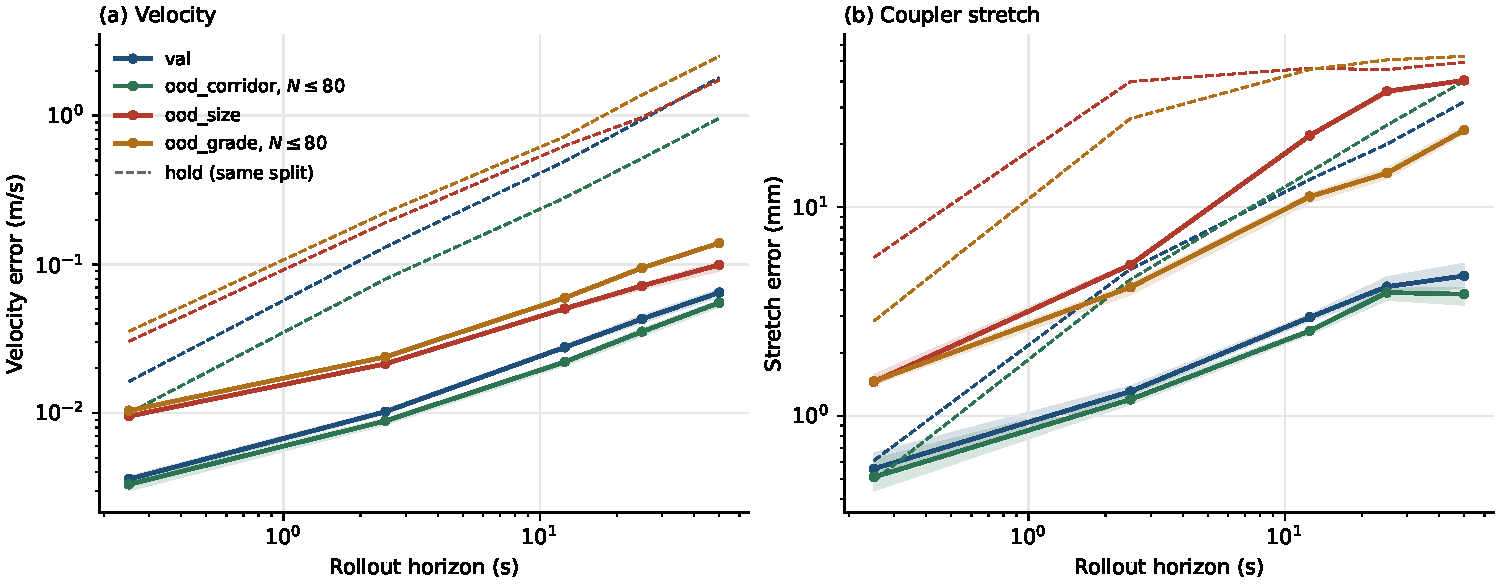
\includegraphics[width=\textwidth]{figures/gns1_rollout.pdf}
    \caption{Rollout error against horizon on four splits, on logarithmic axes. Solid lines are the model (mean over three seeds, with the range over seeds shaded). Dashed lines are holding the starting state on the same split. (a) Velocity error stays more than an order of magnitude below holding on every split. (b) Stretch error does too on \texttt{val} and on the unseen corridor, but on long consists (\texttt{ood\_size}) it rises to meet the holding baseline.}
    \label{fig:train_rollout}
\end{figure}

\subsection{Longer consists}

The test the graph formulation was chosen for is \texttt{ood\_size}: consists of 121 to 150 vehicles, 1.5 to 15 times longer than anything in training, with no overlap. For velocity the result is clear. One-step error rises from 0.015 to 0.022\,m/s$^2$ while the gain over zero output holds at 8.5 times, and after 200 steps the velocity error of 0.099\,m/s (0.090 to 0.106 over seeds) is 18 times smaller than holding the state. Nothing in the model knows how many vehicles there are. Message passing applies the same weights to every vehicle and coupler, and the velocity result is that property working as intended.

For coupler shape the result is the opposite. The one-step correction is still 2.2 times better than zero output, but after 200 steps the stretch error is 40.5\,mm against 49.5\,mm for holding, a gain of only 1.2 times, against 6.8 times on \texttt{val}. The three seeds agree to within 0.2\,mm, so this is a property of the model, not of one run. \Cref{sec:train_shape} examines why.

\subsection{An unseen corridor, and a steep one}

On \texttt{ood\_corridor} at the trained consist lengths, the model is as accurate as in distribution in every column of \cref{tab:train_one_step,tab:train_rollout}, and slightly better on stretch: 3.8\,mm after 200 steps, against 4.7\,mm on \texttt{val}. Generalization to an unseen corridor holds here. Its evidence is one corridor, \texttt{route\_line5}, whose grades are similar to the training corridors (\cref{tab:route_grade_stats_v2}). Including the long consists of the same corridor raises the stretch error after 200 steps to 9.3\,mm, which is the length effect of the previous subsection appearing in a different split. One seed's one-step acceleration error on the full split, 0.032\,m/s$^2$ against 0.020 and 0.019 for the other two, comes from those long consists as well.

On \texttt{ood\_grade} the errors are about twice the in-distribution values at the trained lengths: 0.139\,m/s and 23\,mm after 200 steps, still 18 and 2.3 times better than holding. This corridor is the steepest of the five, with an rms grade of 2.46\% against 0.83 to 1.03\% for the others. The model extrapolates to it, but with clearly degraded accuracy, and its stretch error is closer to the long-consist result than to the in-distribution one.

\subsection{Against constant acceleration}

Constant acceleration is a stronger baseline than its one-step root-mean-square error suggests. On the median of the largest velocity error after one step, it beats the model in distribution by about four times: 0.0009 against 0.0036\,m/s on \texttt{val}. Over most 0.25\,s steps a freight consist's acceleration barely changes, and repeating the last one is very nearly exact. The model's one-step error on those quiet steps sits at about the level of the noise it was trained with. Its advantage lies in the tail, in notch changes, brake applications and slack events, where constant acceleration is badly wrong, and that is why the root-mean-square comparison favours the model by 3.7 times. On long consists, where the tail is larger, the model wins even on the one-step median; on the steep corridor at the trained lengths the two are close.

Rolled out, the comparison is not close. By 10 steps the model's velocity error is three times smaller in distribution, and by 200 steps 21 times smaller. Constant acceleration repeats the last stretch correction as well, and that integrates without bound: its stretch error reaches about 130\,mm after 50 steps on \texttt{val} and about 2\,m after 200. Constant acceleration is a good predictor of the next quarter-second and useless beyond a few seconds, which is the horizon a controller needs.

\section{Coupler shape on long consists}
\label{sec:train_shape}

The one place the model fails to extrapolate is coupler shape on long consists over long horizons. Because the control problem constrains coupler force on long consists over long horizons, this failure matters more than its place in a table suggests, and it was examined in detail. Three hypotheses were tested and rejected. The tests were development runs with one to three seeds and are reported as such.

\subsection{What the error is}

\Cref{tab:train_shape_profile} decomposes the signed per-coupler stretch error over a 200-step rollout on one validation consist of 38 vehicles and one \texttt{ood\_size} consist of 150. Three features matter. The error grows with the number of steps as $n^{0.66}$ on the long consist, faster than the $n^{0.5}$ of independent errors, so successive errors are correlated. Its mean is a quarter of its root-mean-square value. And it is spread evenly along the consist, if anything slightly lower at the rear.

\begin{table}[htbp]
    \centering
    \small
    \begin{tabular}{lcc}
        \toprule
         & \texttt{val}, $N = 38$ & \texttt{ood\_size}, $N = 150$ \\
        \midrule
        Growth exponent ($\text{rms} \propto n^{p}$) & 0.37 & \textbf{0.66} \\
        Bias at 200 steps & +0.15\,mm (2.8\% of rms) & \textbf{+3.91\,mm (26\%)} \\
        Standard deviation at 200 steps & 5.47\,mm & 14.73\,mm \\
        Mean absolute error by quarter (mm) & 1.28 / 1.25 / 1.39 / 1.90 & 11.4 / 8.8 / 10.8 / 6.8 \\
        \bottomrule
    \end{tabular}
    \caption{The signed per-coupler stretch error after a 200-step rollout, on a short and a long consist. The last row gives the mean absolute error in each quarter of the consist, front to rear.}
    \label{tab:train_shape_profile}
\end{table}

\textbf{Not a question of reach.} If five rounds of message passing were too few to coordinate a long consist, the error would grow towards the far end of the train. It does not, so adding rounds for long consists, the first remedy considered, would not have helped.

\subsection{A constraint that should have helped, and did not}

The stretches of a consist are not independent. Their sum is fixed by the positions of the end vehicles, which the trapezoid carries accurately (\cref{tab:arch_position_split}), so the true consist-mean of the stretch corrections is tiny: a standard deviation of 0.026\,mm on training data and 0.008\,mm on \texttt{ood\_size}, against 1.04\,mm per coupler. It is tightest on long consists, exactly where the drift appeared, and the bias in \cref{tab:train_shape_profile} suggested that constraining the edge head to a zero consist-mean would remove it.

\begin{table}[htbp]
    \centering
    \begin{tabular}{lcccc}
        \toprule
        Seed & \texttt{val}, constrained & \texttt{val}, free & \texttt{ood\_size}, constrained & \texttt{ood\_size}, free \\
        \midrule
        0 & 10.12 & 5.84 & 41.06 & 40.96 \\
        1 & 6.48  & 4.42 & 41.49 & 40.41 \\
        2 & 5.31  & 4.60 & 35.42 & 36.65 \\
        \midrule
        Mean & 7.30 & \textbf{4.95} & 39.32 & 39.34 \\
        \bottomrule
    \end{tabular}
    \caption{Stretch error at 200 steps in mm, with the edge head constrained to a zero consist-mean and without. Three seeds.}
    \label{tab:train_zero_mean}
\end{table}

It did not (\cref{tab:train_zero_mean}). The constraint made validation error worse by about half in every seed and left \texttt{ood\_size} unchanged. The mistake was to read a bias of 26\% of the root-mean-square error as 26\% of the problem. The root-mean-square error is $\sqrt{3.91^{2} + 14.73^{2}} = 15.24$\,mm, and removing the bias entirely takes it to 14.73\,mm, a 3\% improvement; the dominant term is variance, and that was visible in the decomposition before any code was written. Why the constraint actively hurts is less certain. Centring couples every coupler's gradient to every other, which plausibly costs more than the freed drift mode gains.

\subsection{Velocity error is not the cause}

Stretch integrates the difference of neighbouring velocities, so a spatially correlated component of velocity error would accumulate directly into shape error, and would also explain the correlated growth. That hypothesis was tested causally rather than by correlation: one channel was forced to the truth at every step of a rollout, and the error of the other was measured.

\begin{table}[htbp]
    \centering
    \begin{tabular}{lcc}
        \toprule
        Rollout & \texttt{val}, $N = 38$ & \texttt{ood\_size}, $N = 150$ \\
        \midrule
        Model on its own output         & 1.27\,mm & 44.18\,mm \\
        True velocity forced every step & 1.73\,mm & 40.07\,mm \\
        \bottomrule
    \end{tabular}
    \caption{Stretch error at 200 steps with and without the true velocity field forced into the rollout.}
    \label{tab:train_shape_oracle}
\end{table}

A perfect velocity field removes 9\% of the shape error on the long consist, and on the short one it makes shape \emph{worse} (\cref{tab:train_shape_oracle}). The reverse holds too: forcing the true stretch raises the velocity error on \texttt{ood\_size} from 0.083 to 0.139\,m/s. The two channels' errors are anti-correlated. The model has learned a self-consistent effective dynamics in which its velocity and stretch errors partly cancel, and forcing the truth into either breaks that compensation. One general consequence follows: a test that scores one channel against a teacher-forced other understates how good the joint state is.

\subsection{A failure of stability, not accuracy}

The per-step correction error on \texttt{ood\_size} is only 17\% larger than on validation, yet after 200 steps the stretch error is about 35 times larger in the same comparison. The difference is in how errors accumulate. On validation the rollout accumulates less error than a random walk of the same per-step size would, about 1.3\,mm against 5.7\,mm, so errors correct themselves. On \texttt{ood\_size} it accumulates more, about 44\,mm against 22\,mm, so errors reinforce one another. The learned dynamics is a stable attractor within the training range of consist sizes and not outside it.

Two hypotheses about the model have been rejected and a third, more message passing, was ruled out by the error profile before it was tried. Without an idea aimed specifically at stability, further changes to the model were not pursued in Part~I. The practical consequence is a separation of claims: velocity extrapolates to unseen consist lengths, coupler shape over long horizons does not, and a controller that needs coupler force on long consists should be given a model trained on the consist sizes it will control.

\section{Cost of a step}
\label{sec:train_cost}

\Cref{sec:arch_step} gave the surrogate's structural saving: one network evaluation replaces the fifty right-hand-side evaluations the reference integrator makes between two stored states. That ratio is fixed by the integrator's configuration. Wall clock is a separate question, and it was measured on the workload of \cref{tab:gpu_throughput}: 120\,s of simulated time, 480 output steps, for consists of 130 vehicles from \texttt{ood\_size}. The timing covers the whole rollout loop, including feature construction, route lookup and the state update.

\begin{table}[htbp]
    \centering
    \begin{tabular}{rcccc}
        \toprule
        $B$ & GNS-1 & Integrator, single & Integrator, double & GNS-1 per scenario \\
        \midrule
        1   & 1.78\,s & 3.28\,s & --- & 1,780\,ms \\
        64  & 1.68\,s & 3.71\,s & 5.03\,s & 26\,ms \\
        256 & 3.27\,s & 4.01\,s & 5.49\,s & 13\,ms \\
        \bottomrule
    \end{tabular}
    \caption{Wall clock for 120\,s of simulated time at $N = 130$ on one RTX~4090: GNS-1 rolled out in plain PyTorch, against the GPU integrator replayed as a CUDA graph in single and in double precision (\cref{tab:gpu_throughput,tab:gpu_precision}). The corpora were integrated in double precision.}
    \label{tab:train_cost}
\end{table}

The fifty-to-one ratio does not become a fifty-fold saving in time (\cref{tab:train_cost}). The surrogate is 1.2 to 2.2 times faster than the integrator in single precision, and 1.7 to 3.0 times faster than the double-precision integration the corpora were built with. The reason is the one \cref{sec:gpu_throughput} found for the integrator itself: on this GPU both are limited by the overhead of issuing each step, not by arithmetic. The integrator replays each step as one recorded CUDA graph; the surrogate, as measured, launches every operation of every step separately. Recording the surrogate's step the same way is the obvious next optimization and was not done in Part~I. Against the NumPy reference simulator, which needs at least 89.2\,s for the same scenario on one core, a single surrogate rollout is about 50 times faster.

The speed claim of Part~I is therefore the structural one: fifty evaluations become one. Measured wall clock confirms a saving, but a modest one, and it depends more on implementation than on the formulation.

\section{What Part~I claims}
\label{sec:train_claims}

\Cref{tab:train_claims} lists what this chapter's results claim, each with its evidence. The third column names what the claim rests on beyond the measurement itself. \Cref{ch:critique} examines those foundations and marks each claim as standing, qualified or withdrawn, and \cref{ch:results2} marks them again for the rebuilt system.

\begin{table}[htbp]
    \centering
    \small
    \begin{tabular}{>{\raggedright}p{0.6cm}>{\raggedright}p{4.6cm}>{\raggedright}p{4.4cm}>{\raggedright\arraybackslash}p{3.4cm}}
        \toprule
        & Claim & Evidence & Rests on \\
        \midrule
        C1 & The network learns the 0.25\,s step. & Mean acceleration RMSE 0.015--0.019\,m/s$^2$ in distribution, 7.3--7.5$\times$ zero output, 3.7--3.8$\times$ constant acceleration (\cref{tab:train_one_step}). & The simulator as the definition of truth. \\
        C2 & With noise injection and pushforward, rollouts stay accurate over 200 steps (50\,s). & 0.065\,m/s and 4.7\,mm after 200 steps on \texttt{val}, 28$\times$ and 6.8$\times$ better than holding (\cref{tab:train_rollout}). & Development sweeps on one seed (\cref{tab:train_noise_sweep,tab:train_push_sweep}). \\
        C3 & Velocity extrapolates to consists 1.5--15$\times$ longer than any trained on. & 0.099\,m/s after 200 steps on \texttt{ood\_size}, 18$\times$ better than holding; one-step gain 8.5$\times$ zero output. & Consist library and couplers of the legacy simulator. \\
        C4 & Coupler shape does \emph{not} extrapolate to long consists over long horizons. & 40.5\,mm against 49.5\,mm for holding after 200 steps, 1.2$\times$, consistent over seeds; diagnosed as instability (\cref{sec:train_shape}). & The Kelvin--Voigt coupler with deadband. \\
        C5 & The model generalizes to an unseen corridor. & At trained lengths, \texttt{ood\_corridor} matches in-distribution accuracy (0.055\,m/s, 3.8\,mm after 200 steps). & One corridor, of grades similar to training. \\
        C6 & The model extrapolates to steeper terrain, with degraded accuracy. & \texttt{ood\_grade} errors about twice in distribution; 18$\times$ and 2.3$\times$ better than holding. & The grade field of \texttt{route\_line2}. \\
        C7 & One network evaluation replaces fifty right-hand-side evaluations. & Integrator configuration (\cref{sec:gpu_port}); measured wall clock 1.2--3.0$\times$ faster than the GPU integrator (\cref{tab:train_cost}). & Integrator step of 0.02\,s. \\
        \bottomrule
    \end{tabular}
    \caption{What Part~I claims. \Cref{ch:critique} examines the third column.}
    \label{tab:train_claims}
\end{table}

All seven claims are about the surrogate's fidelity to the simulator that generated its data, not about fidelity to a real train. That distinction, stated in \cref{ch:refsim}, is where Part~II begins.

\section{Chapter summary}

The graph network simulator of \cref{ch:architecture} was trained on \texttt{data/v2} across every consist size from 10 to 80, in batches of a single size so that no padding is needed. Trained only to predict one step, it diverged within about 20 steps of a rollout. Injecting noise into its training inputs, with targets recomputed to the true next state, made it stable, and adding three pushforward steps improved it further; the two work together and neither replaces the other.

Over three seeds, the trained model predicts the step 7.5 times better than zero output and stays accurate over 200 steps, 50\,s of simulated time, at 0.065\,m/s in velocity and 4.7\,mm in coupler stretch. Its velocity predictions extrapolate to consists up to 15 times longer than any it was trained on, and to an unseen corridor at full accuracy. Its coupler shape predictions do not extrapolate to long consists over long horizons, a failure traced to the stability of the learned dynamics rather than to its per-step accuracy or to velocity error. On the steepest corridor its errors double. A rollout costs one network evaluation per stored step instead of fifty, which on this hardware and implementation is a 1.2 to 3 times saving in wall clock.

These are the results of the first experiment, and \cref{tab:train_claims} states them as claims. Every one of them is measured against the simulator that produced the data. The next part of the thesis asks how far that simulator, and the routes and data built on it, can be trusted.
